\chapter{POTENTIAL DEVELOPMENT SOFTWARE}
\label{ch:software}

\section{Introduction}

The simulation of atoms involving hundreds of atoms are commonplace, due to the success of density functional theory\cite{hohenberg1964_dft,kohn1965_dft} and the availability of many software packages avail for the calculations such as VASP\cite{kresse1993_vasp,kresse1996_vasp1,kresse1996_vasp2}, ABINIT\cite{gonze2002_abinit,gonze2005_abinit,gonze2009_abinit,gonze2016_abinit}, and Quantum Espresso\cite{giannozzi2009_quantumespresso}.  
These electronic-structure calculations are high-fidelity calculations, which accuracy improving as the description of the exchange correlation energy functional has improved from local density approximation(LDA) to PBE to hybrid methods.
These electronic-structure models allow for simulations of hundreds of atoms which when combined with workflow management software, such as \emph{AFLOW}\cite{curtarolo2012_aflow} and \emph{pymatgen}\cite{ong2013_pymatgen} has given rise to high-throughput computational efforts, which leverage these energy calculators.

As an alternate to electronic structure methods, the use of empirical potentials that describe the effects of the valence electron interactions without explicitly describing the electrons themselves.  The simplied descriptions of interatomic interations allow for larger system sizes and longer simulations timeframes than can be accomplished with \emph{ab initio} techniques.  However, these approaches are accompanied by a loss of accuracy compared to electronic structure methods.

In this chapter, a software toolkit for the reproducible, algorithmic development of interatomic potentials for atomic-level simulations using autonomous machine-learning techniques is described.
The Python Potential Optimization Software Package (\emph{PyPOSPack}) is open-access software for the automation of potential development workflows, which leverages the richness of machine learning codes of the python language with ubiquitous molecular dynamics software code, LAMMPS\cite{plimpton1995_lammps}, and the lattice dynamics code, GULP\cite{gale2003_gulp}.

\subsection{Current state of Potential Development Software}

Classical atomistic simulation methods, of which molecular dynamics (MD) simulation\cite{allen1987_md,haile1992_md,lesar2013_md,frenkel2002_md} is the most common, are a vital tool in the analysis of solid state and materials systems.
The description of the interactions of the atoms is encoded in the interatomic potential, many of which have been developed to describe specific materials systems.
The embedded atom method (EAM)\cite{daw1983_eam,daw1984_eam,daw1993_eam_review,foiles2012_eam_review} and Finnis and Sinclair\cite{finnis1984_fs} potentials, among others, were developed and continue to be developed for metals.
Bond order potentials (BOP) such as those of Brenner\cite{brenner1989_bop,brenner2002_rebo} and Tersoff\cite{tersoff1988_tersoff}, and the three-body Stillinger and Weber\cite{stillinger1985_sw} potential are widely used to describe covalently-bonded materials.
For ionically bonded materials, the electrostatic interactions are typically described by Coulomb potentials, with various formalisms for the short ranged interactions, the Buckingham potential being the most widely used.\cite{lewis1985_buck,gale1996_buck}
The continuing evolution of these formalisms, the development of more sophisticated potential formulations such as ReaxFF\cite{vanduin2001_reaxff,senftle2016_reaxff} and COMB \cite{liang2013_comb_1,liang2013_comb_2}, and the increasing accuracy of density functional theory (DFT) calculations, which typically constitute at least part of the fitting database, have allowed the materials fidelity of these potentials to increase markedly.

\begin{figure}[ht]
	\label{fig:potdev_monolithic}
	\centering
	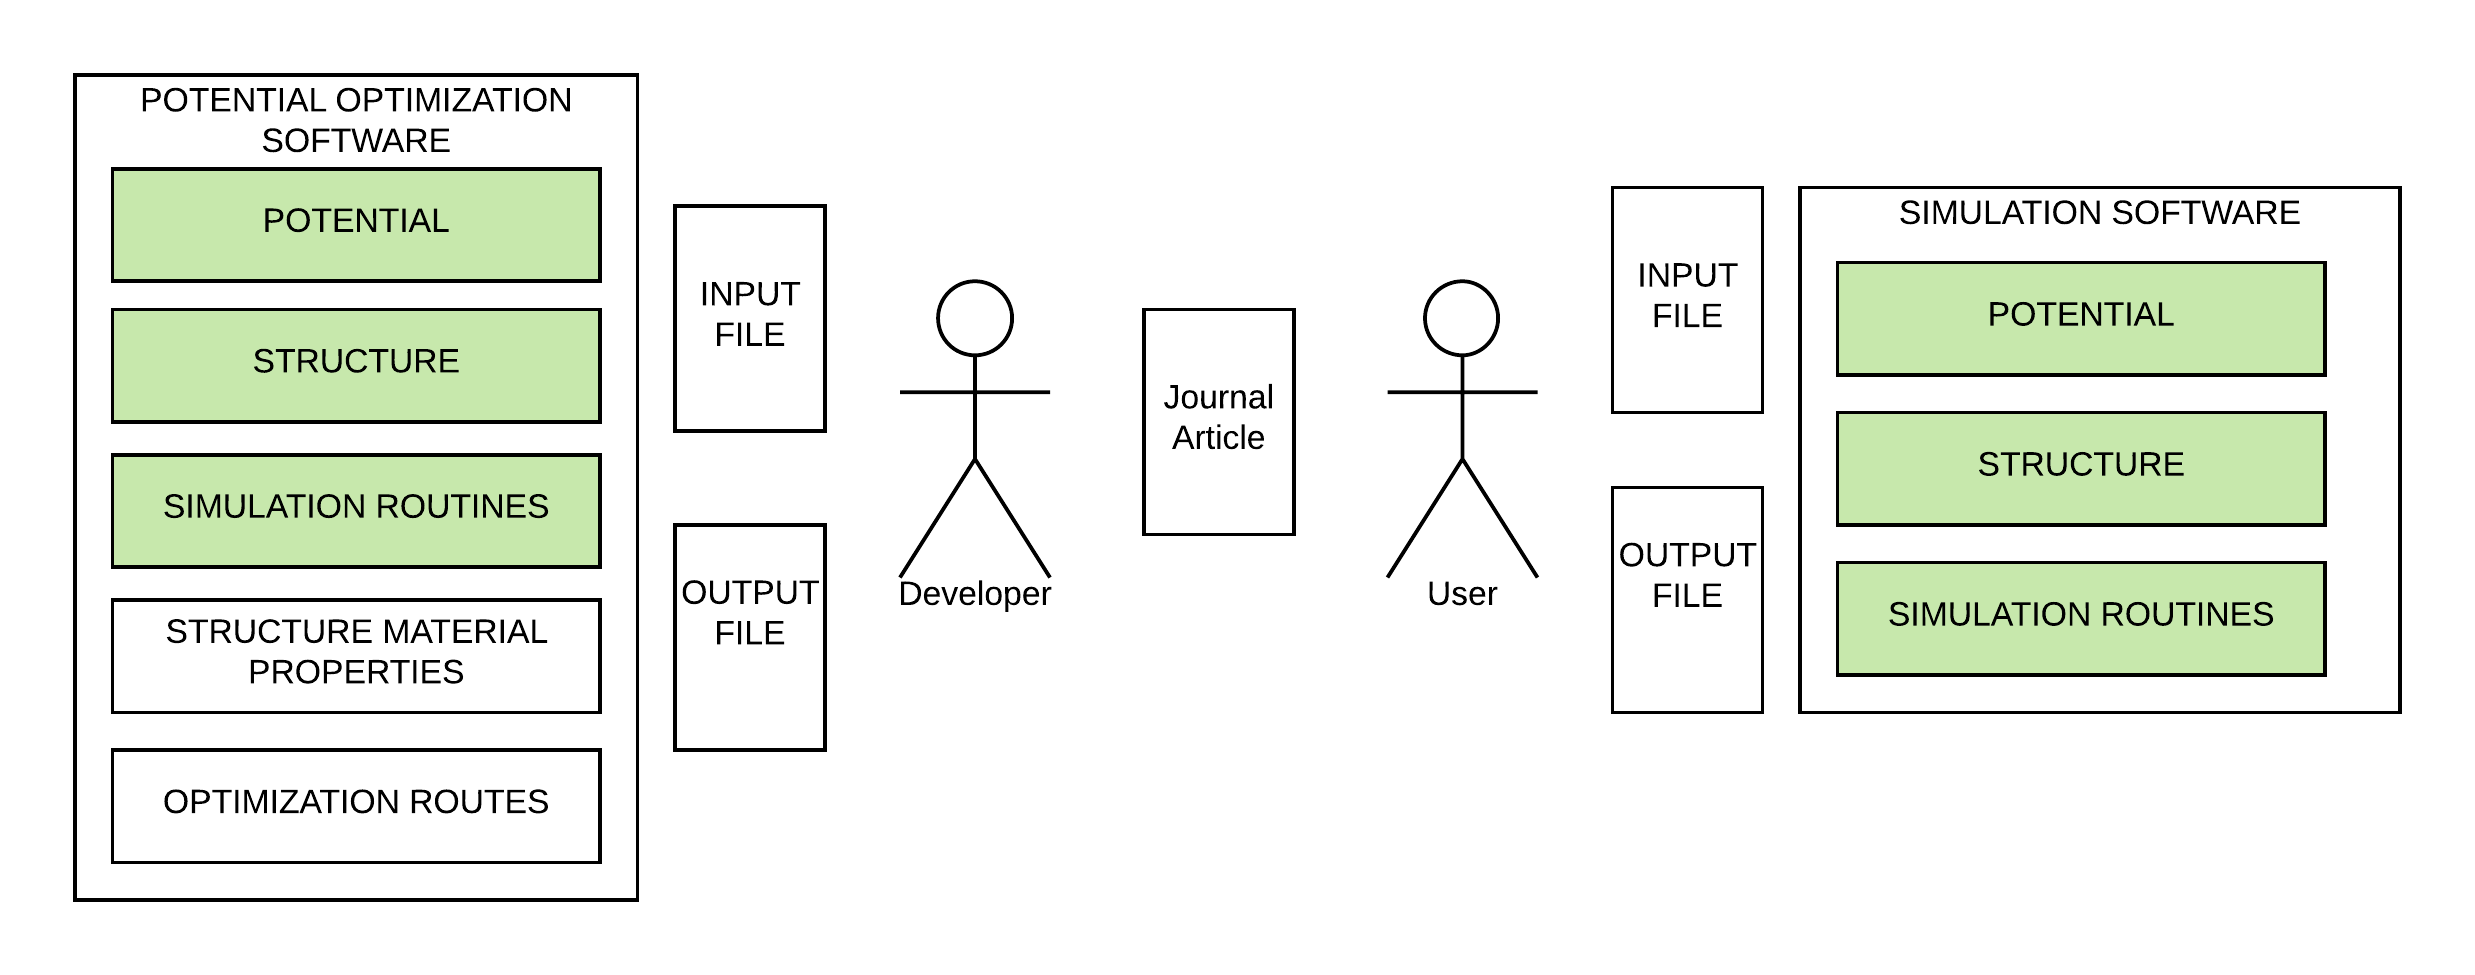
\includegraphics[width=5in]{chapter6/img/fig_potdev_monolithic}
	\caption{Schematic of monolithic potential development software}
\end{figure}

Figure \ref{fig:potdev_monolithic} is a schematic between potential development software, simulation software, the potential developer, and the potential user.  In this software architecture, The code for implementing the potential, the structures, and simulation routines common to molecular dynamics software.  

Computational atomistic simulation involves software which have been developed in a variety of different languages, including but not exclusive to C/C++, and Fortran.  The combination of compiler optimization from strict variable types, well-vetted numerical libraries, and availability of parallelization libraries makes these langagues well-entrenched for the forseeable future.  The most popular atomistic simulation codes have matured over long-periods of time, with significant code contributions from the developers of potential formalisms enhancing the capabilities of the software.  For example, LAMMPS was originally written in Fortran, ported to C/C++.  

Similarly, potential development software likewise developed iteratively, but with drastically different results.  Early potentials were developed using proprietary simulation codes which were augmented to describe the ability to describe the specific set of simulations to conduct required to optimize a specific set of simulations to calculate structure-property relationships.   In addition, numerical optimization routines to minimize a cost function as described in chapter \ref{ch:potential_development}.  Software codes included the ability to assign weights to the function to encode preferences and evolved to include global optimization techniques, such as simulated annealing\cite{kirkpatrick1983_simmulated_annealing} to deal with the local minima.

Despite the drastic expansion in the amount of formalisms and maturation of simulation codes, potential development software remains tailored to specific potentials and applications.  Potential software was written which support a small subset of potential formalisms.  For example, \emph{POSmat}\cite{martinez2016_posmat} supports the development of COMB potential and \emph{potfit}\cite{brommer2015_potfit} supports the development of embedded atom potentials (EAM).  On the other hand, GULP supports development of potentials based on a relatively small set of material properties.   

The monolithic software development model is ill-suited for the demands of potential development.  As indicated in Figure \ref{fig:potdev_monolithic}, the regions in green represents a replication in development effort with simulation codes.  The implementation, maintenance, and updating of molecular dynamics code is non-trivial.  This effort is duplicated and better implemented in widely-adopted software codes such as LAMMPS.  More importantly,  there is little incentive for a third-parties to implement new potential formalism to monolithic software development codes.

Discussed in depth in chapter \ref{ch:potential_development}, the final parameterization on depends choices made by the potential developer; this means that the process by which a potential is developed is generally neither fully documented, nor reproducible.  Moreover, there is currently no objective method for evaluating the suitability of the function form of the atomic potential or determining if the final parameterization selected yields the best possible fit to the fitting database.  Current parameterization processes generally involve the minimization of a single scalar cost function, typically a weight sum of some measure of the predicted value, $\hat{q}_i(\bm{\theta})$ and the reference values of the specific material property $\hat{q}_i$.

As a result, the final parameterization depends on the many choices made by the potential developer; this means that the process by which a potential is developed is generally neither fully documented, nor reproducible.  Nevertheless, the process of potential development largely remains non-transparent and subjective,\cite{martinez2013_fitting,martinez2016_posmat} involving the repeated intervention of a skilled potential developer.\cite{brenner2000_fitting}
This leads to issues to problems with reproducibility in potential development as the selection of weights and initial conditions are largely not documented with the literature.  
As a result, this knowledge is largely proprietary, remains concentrated in potential development groups, and software for potential development remain rudimentary tools developed by the specific needs of potential development groups.

In addition, parameter optimization is dependent upon numerical optimization techniques indicated in orange in Figure \ref{fig:potdev_monolithic}.  As described by Ghosh and Chakraborty \cite{ghosh2014_potdev_pareto}, the general problem of parameterization is a classic problem in the application of black box functions.  Cost function optimization techniques are unable to obtain compromise solutions which are Pareto efficient, but are occluded within a convex region of performance space.  

\subsection{Goals of this Software}

The key driver of this software is to implement a systematic methodology to fit interatomic potentials that allows the objective evaluation of the quality of the parameterization, and the stability of the functional form, and that is both completely algorithmic and reproducible.  

Like other potential development software packages, \emph{PyPOSPack} was developed to seprate the process of parameter optimization from the selection of the analytical form of the potental.  \emph{PyPOSPack} separates itself from other packages by designed using object-oriented methods which enables users of this software to quickly integrate new potentials, material properties, or even optimization techniques.

This software developed from a driving interest of exploring parametric uncertainty of interatomic potentials described by analytic functional forms. which required the incorporation of multiple potentials, simulation of different material properties, and different optimation options.  Here, we assume that a potential is already implemented in LAMMPS.  Rather than searching for computational efficiency and accuracy by replicating code already implemented in simulation.  As a result, LAMMPS remains largely a procedural software development program.  Here, computational efficiency is secondary to easy of developent.  The evaluation of a parameter is largely dependent upon the costs of the simulation, which is sent to an external calculator such as LAMMPS or GULP, and we choose Python as programming language of choice.

In the primary use case, the potential developer will look to approximate the parameter set which produces Pareto optimal predictions.  Since parameter space is explored by sampling from a probability distribution, this effort is embarassingly parallelizable and we wish to scale this effort over the large number of processors available in a high performance cluster (HPC) environment likely available to potential development.  The typical use case for this software package involves a potential developer using the software program by modifying the examples distributed with this program for their particular needs.

More generally, the secondary goal of this software project is to implement the necessary architecture for potential developers to write their own potential development software, either by extending the base the class to include more potential formalisms, simulations tasks, and calculation of material properties.  As a result, specific software architecture decisions were made to decouple the base classes from each other.

In general, this software focuses on the integration of other software.  It interacts with other software packages, but is loosely coupled by encapsulating interation of that software through an integration layer of objects.  In this way, it is possible to change the third party software dependencies by the implementation of a new integration layer.  Despite this loose coupling, great care was taken to ensure the selection of prominent softwre packages.  The benefits of using widely-accepted existing software include avoiding the mistakes involved from self-implementation, saving development effort, and that the underlying routines have sufficient documentation and support.

Software for potential software development is by necessity a complicated piece of software which draws expertise from many disciplines for software development.  The goal of pypospack is not to deliver a monolithic software application, but provide a software with a flexible software architectural library from which potential developers can quickly create their own potential optimziation software, by leveraging an object-orient software framework based upon a series of core packages, which deliver specific functionality to \emph{PyPOSPack}.

\subsection{Structure of this chapter}

This chapter starts by first discussing architectural considerations taken into account in the development of this software library.  Section \ref{sec:software_architecture} includes language selection, incorporation of prominent software packages, and core design choices which has implication for the use of this software package.  At the heart of the problem is the implementation of potentials, structures, and material properties which are described first.

Section \ref{sec:potential_evalaution} deals with the generalizing the calculation of material properties.  The calculation of material properties is often decomposed into several different simulations, the simulations executed, and the results gathered.  With the results from the individual components calculated, the material property of interest can then be calculated.  This section describes how this model decomposition is implemented and the execution framework evaluating a single parameter.

Both of these sections implements concepts introduced in Chapter \ref{ch:potential_development} and reuses the notation.  With the evaluation of a single parameter set accomplished, Section \ref{sec:software_sampling_strategies} describes implementation of the evolutionary strategy described in Chapter \ref{ch:methodology}.  In addition, to a discussion of the types of strategies implemented, this section specfically discusses how computational scalability is achieved by resolving concurrency and parallelization issues to ineable this software's use in high-performance computing environments.

While older monolithic codes have terse input and output files, the issues of accessibility to software in \emph{PyPOSPack} are resolved through the concept of object serialization and deserialization.  Section \ref{sec:softwre_acessibility} describes this strategy.  Since every object in \emph{PyPOSpack} can be instanced by a dictionary datastructure, the definition of an optimization process can be represented as a nested list of dictionaries.  This enables potential developers to define evolutionary strategies quite compactly, since the the deserialization results of the previous interation are used to serialized the next iteration.

Section \ref{sec:software_analysis}, we demonstrate the power of this framework, by looking at how the large amounts of data produced by simulation methodology is readily available to potential developer using well-known data analysis tools.  With the removal of traditional input and output files, the large amounts of data generated are readily accessible and accessible for exploratory data analysis.

\section{Software Architecture}
\label{sec:software_architecture}

\emph{PyPOSPack} is written in Python 3 to leverage the strength of python as a high-level language for writing scientific applications.  Python has a liberal open source license which makes the distribution of the application without license issues.  Compatability across platforms is a major design consideration.  Since Python available of a wide variety of operating systems, there are few issues with portability as \emph{PyPOSPack} is written to be platform agnostic.

\emph{PyPOSPack} utilizes prominent open-source packages from the python community.  Python is popular programming language that is popular for scientific applications, due to the maturity and stability of fundamental numerical libraries, quality of documentation, and availability of well-supported distrbutions, such as Anaconda\cite{python_anaconda}, makes Python accessible and convenient for a broad audience.  Additionally, matplotlib\cite{hunter2007_matplotlib} integrated with IPython\cite{} provides an interactive research and development environment with data visualization suitable for most users.  As a result, is an appealing choice for algorithmic development and exploratory data analysis\cite{dubois2007_python}

Since, \emph{PyPOSPack} takes a different approach to the development of potentials by identifying a set of Pareto optimal potentials through an evolutionary process.  NumPy\cite{walt2011_numpy} adds an array language, similar in syntax to MATLAB, and similar in power to Fortran, in which operations are performed in compiled code.  This package provides linear algebra capabilities through this extended interfaces to BLAS\cite{blas2002} and LAPACK\cite{anderson1990_lapack}.  Scipy\cite{jones_scipy} builds on top of NumPy to provide functionality for optimization, numerical integration, and a statistics package for creating random variates.

The python language has a clean syntax yet has sophisticated constructs which allows is indifferent to either procedural or object-oriented programming styles, as the situation dicates.  Software development for this program was developed using procedural code, which was later encapsulated to classs object to abstract the implementation details into base objects.  The success of \emph{pymatgen} in transforming the high-throughput search of materials,  where the materials properties can be predicted by solving fundamental laws of physics using quantum mechanical appoximation such as density functional theory (DFT).  This virtual testing of materials was employed to design and optimize materials \emph{in silico}.

For the purposes of data analysis, the data produced by \emph{PyPOSPack} is exposed through Pandas\cite{mckinney2010_pandas} to simplify data management and data analysis tasks using well known syntax.
Scikit-learn\cite{pedregosa2011_sklearn} integrates a wide range of machine learning algorithms for medium-scale supervised and unsupervised problems. This package focuses on bringing machine learning to non-specialists using a general-purpose high-level language.

Scalability for \emph{PyPOSPack} is provided through the MPI for Python(mpi4py(\cite{dalcin2005_mpi4py,dalcin2008_mpi4py} which provides bindings of the Message Passing Interface (MPI)\cite{mpi2015} standard for the Python programming language and allows the exploitation of multiple processors in an HPC environment.  This is important for ease of installation and portability, as providing libraries around Fortran code can prove challenging on various platforms.
\subsection{External Simulation Codes}

\emph{metal} units, where further information can be found in the LAMMPS 

\subsection{Potential Formalisms}

The software development effort associated with developing new potentials for potential optimization software is typically time-consuming, requiring the implementation not only of the potential $\hat{V}$ but also the implementation of the second-derivatives with respect to changes in interatomic positions to computational issues with numerical approximation.  In \emph{PyPOSPack}, this requirement has already been implemented by the simulation software, which drastically reduces the software development time to implement existing formalisms already supported by either LAMMPS or GULP.

The \verb|potential| package contains class objects which inherit from the appropriate abstract base class and overide the required methods for implementation.  The \verb|Potential| abstract class only expects implementation of the \verb|_init_parameter_names|, \verb|lammps_potential_section_to_string|, \verb|gulp_potential_section_to_string|, \verb|lammps_parameter_file_to_string| and \verb|evaluate| methods.  However, not each method needs to be implemented.  

Depending upon the use of the potential, not all methods need to be overridden.  For example, if simuations are only run in LAMMPS, then the only the \verb|lammps_potential_section_to_string| would need to be implemented  to be implemented respectively.

In \emph{PyPOSPack}, the \verb|potential| package contains classs objects, which inherit from methods from the appropriate base class.  The base classes have been implemented in \verb|potential|: (1) \verb|PairPotential|, (2) \verb|ThreeBodyPotential|, (3) \verb|EamDensityFunction|, and (4) \verb|EamEmbeddingFunction|.  

The base potentials implement a standard potential naming scheme.  For example, for a pair potential with a parameter, $A_{Mg,O}$, satifies the $A$ parameter of the Mg-O pair potential term, and would have the name \verb|MgO_A|.  As a result, it is necessary only to define the \verb|pair_parameter_names| attribute in implemented potential classes.  Implemented pair potentials are indicated in Table \ref{tbl:pypospack_pair_potential}. 

\begin{table}[ht]
    \centering
    \caption{Implemented pair potentials in \emph{PyPOSPack}.}
    \label{tbl:pypospack_pair_potential}
    \begin{tabular}{ccccc}
	    \hline
	    {Class Name} & LAMMPS & GULP & EAM  & {Reference} \\
	    \hline
	    BuckinghamPotential   &   &   & x & \cite{lewis1985_buckingham,buckingham1938} \\
	    MorsePotential        & x & x & x & \cite{morse1929_morse_potential} \\
	    BornMayerPotential    &   &   & x & \cite{abrahamson1969_bornmayer_potential} \\
	    LennardJonesPotential & x & x & x & \cite{lennardjones1924_lj_pot} \\
	    GeneralizedLennardJonesPotential
	                          &   &   & x & \cite{mishin2004_eam_NiAl} \\
	    \hline
    \end{tabular}
\end{table}

Three body potentials are implemented in with the base class \verb|ThreeBodyPotential|, and listed in Table \ref{tbl:pypospack_threebody_potentials}.  Unlike pair-potentials, the potential naming schemes are not equivalent.  In the Stillinger-Weber potential\cite{stillinger1985_sw}, a pair potential term $V_2(r_{ij})$ is dependent upon the interatomic separation distance between atoms $r_{ij}$ between atoms $i$ and $j$.  To model angular dependence the three-body term $V_3(r_{ij},r_{ik},\theta_{ijk})$ augments the $V_2$ term, where $i$ is the central atom in a three body interaction.  In comparison, the Tersoff potential\cite{tersoff1988_tersoff} is a pair interaction term describing the bonding of atoms $i$ and $j$ influenced by the presence by a third atom $j$.  In the Tersoff potential, an entry for SiCC means that a silicon atom is bonded to a carbon atom and influenced by a third atom.  Unlike the Stillinger-Weber potential, the three-body parameters for SiCC and SiSiC will not, in general be the same.  As a result, \verb|_init_parameter_names| has different implementations for three-body potentials, and the base class has not default implementation.

\begin{table}[ht]
	\centering
	\caption{Implemented three-body potentials.}
	\label{tbl:pypospack_threebody_potentials}
	\begin{tabular}{cccc}
		\hline
		{Class Name} & LAMMPS & GULP & Reference \\
		\hline
		TersoffPotential & x & x & \cite{tersoff1988_tersoff} \\
		StillingerWeberPotential & x & x &\cite{stillinger1985_sw} \\
		\hline
	\end{tabular}
\end{table}

The formalism of the EAM potential is composed of three functions: (1) a pair potential, (2) an electron density function, and (3) an embedding energy function which is dependent upon individual contributions defined by the electron density function.  
The implementation of the \verb|EamPotential| class encasulates  a \verb|PairPotential|, a \verb|EamEmbeddingFunction|, and a \verb|EamDensityFunction|.  With the abstract for the pair potential already defined, the abstract classes for \verb|EamDensityFunction| and \verb|EamEmbeddingFunction| are used exclusively for the development of analytical embedded atom method (EAM) potentials.

The list of implemented EAM and are listed in Tables \ref{pypospack_eam_density_function}.  A density function $\bar{\rho}(r_{ij})$ is the electron density contribution of atom $j$ to the total electron density at the site for atom $i$.  Like a pair potentia, it is a function the interatomic separation distance.  However, each species is bound to an electron density function.  For an EAM potential with two chemical species, there are two electron density functions.  Thus the parameter naming convention would be \verb|{symbol_1}_{parameter_name}|.

\begin{table}[ht]
	\centering
	\caption{Implemented EAM density functions}
	\begin{tabular}{cc}
		\hline
		{Class Name} & {Reference} \\
		\hline
		ExponentialDensityFunction & \\
		Mishin2004DensityFunction & \cite{mishin2004_eam_NiAl} \\
		\hline
	\end{tabular}{cc}
\end{table}

\emph{PyPOSPack} supports two representations of the embedding function.  The default implementation defines the embedding function, $F(\bar{\rho}|\bm{\theta})$, as regular analytical function.  The analytical function The second representation comes from inversion of the equation of state, a technique pioneered by Foiles \emph{et al.}\cite{foiles1986_eam_embedded_eos}.  The \verb|EamEmbeddingEquationOfState| provides a base class for the numerical estimation of these functions, and are listed in Table \ref{tbl:pypospack_eos_embedding_function}.
\begin{table}[ht]
	\centering
	\caption{Implemented Analytical embedded energy function.}
	\label{tbl:pypospack_embedding_function}
	\begin{tabular}{cc}
		\hline
		{Class Name} & Reference \\
		\hline
		BjsEmbeddingFunction & \\
		UniversalEmbeddingFunction & \\
		FinnisSinclairEmbeddingFunction & \\
		\hline
	\end{tabular}
\end{table}

EAM potentials are not defined in simulation software as analytical potentials, but provided in a pre-calculated tabulated format known as the \emph{setfl} format.  The class \verb|SetflFile| contained in the \verb|eamtools| packages deserializes a parameterized EAM potential into the expected format.

\begin{table}[ht]
	\centering
	\caption{Implemented EAM embedding function determined from the inverse equation of state}
	\label{tbl:pypospack_eos_embedding_function}
	\begin{tabular}{cc}
		\hline
		{Class Name} & {Reference} \\
		\hline
		RoseEosEmbeddingFunction & \cite{foiles1984_eam_eos} \\
		ZopeMishinEosEmbeddingFunction & \cite{zope2003_eam_eos} \\
		\hline
	\end{tabular}
\end{table}




\section{Structural Representation}

The structural representation of 

\section{Potential Evaluation}
\label{sec:potential_evalaution}

To run simulations, \emph{PyPOSPack} spawns a new process, through the Python \verb|subprocess| module, and obtain the exit codes, which is returned from the child process and is interpreted by \verb|pypospack| in the event of external codes returning a success or failure.  Through this facility, input files are made for the external executable, which is run under a child subprocess until an exit code is detected, when the output files of the energy calculator are then parsed for pertinent information.  Currently, \verb|pypospack| supports LAMMPS and GULP as external energy calculators

Software for potential software development is by necessity a complicated piece of software which draws expertise from many disciplines for software development.  The goal of pypospack is not to deliver a monolithic software application, but provide a software with a flexible software architectural library from which potential developers can quickly create their own potential optimziation software, by leveraging an object-orient software framework based upon a series of core packages, which deliver specific functionality to \verb|pypospack|.


\subsection{Simulation Tasks}
At the heart of the \verb|pypospack| conceptualization of the parameterization workflow is the decomposition of the calcuation of material properties into individual simulations.

All tasks inherit from the the abstract class \verb|task.Task|, with an intermediate abstract class for the implementation of simulation tasks for LAMMPS(\verb|AbstractLammpsSimulation|), and GULP(\verb|task.gulp.GulpSimulation|.  LAMMPS and GULP implementation of tasks are determined separately.

A simulation task has several states: INIT, CONFIG, READY, RUNNING, POST, FINISHED, and ERROR.  It start with INIT and proceeds to the other stages unless an error conditions happens, in which case the instance of the class is marked with the status ERROR.

The INIT state is automatically set when a Task is instantiated.
When, the TaskManager provides the information necessary to a class, with exception of information it requires from other tasks, it will mark itself into the CONFIG state, unless it is not dependent upon Task completation, in which case it will automatically move to READY.
When all Tasks reach the CONFIG state, then the TaskManager will begin running simulations by creating a the necessary input files to the external calculator, such as LAMMPS or GULP, subprocess the calculator to run the simulation, and mark the status as RUNNING.
Monitoring of the subprocesses in done within a sleep loop in the TaskManager; the TaskManager iterates throug the list of tasks, instructing it to poll it's subprocess, this enables multiple simulations to be done simultaneously, without locking the main thread.  Each task with logic to identify abnormal exit conditions of the simulation software and will kill the child subprocess, without killing the main thread.
When the simulation is complete, the Task will notice that the subprocess is complete TaskManager will then mark the task in being the POST state, indicating that the results of the simulation are ready for post-processing.  The task manager will then instruct the task to post-process the results of the simulation by reading the output files and providing the information as dictionary object which is then broadcast to all the other tasks as well as the QoiManager, which collects the data for the calculation of material properties.  When the post-processing tasks are complete and the information received by the TaskManager, the task is then marked FINISHED.

When all tasks have the FINISHED status, then all simulations are complete, and the information is transferred from the TaskManager to the QoiManager for calculation of material properties.

\subsection{Defining Material Properties}

\section{Sampling Strategies}
\label{sec:software_sampling_strategies}

\section{Accessibility}
\label{sec:softwre_acessibility}

\section{Analysis and Visualization}
\label{sec:software_analysis}
\subsection{Object serialization and deserialization}

Pypospack makes extensive use of object serialization, by encapsulating pertinent information into a data structure of key-value pairs.  
Known more generally as a hashtable, collections of key-value pairs are implemented in Python as a data structure called a dictionary (i.e. \verb|dict| or \verb|OrderedDict|).  
Every object within \emph{pypospack} can be instantiated in different ways: by default constructor, by dictionary constructor, and through object serialization.   
For a object called \verb|ObjectName|, arguments are passed to the object's default constructor, \verb|ObjectName.__init__(self, args, kwargs)|.  
Here \verb|args| are mandatory and order-dependent arguments, and \verb|kwargs| are optional arguments used to modify default behavior.  
Due to the complexity of these classes, all implemented objects are required to override the abstract method of the base class, \verb|ObjectName.init_from_dict(d)|, which is a static factory method which takes a dictionary of arguments and parameters and returns an object.  More importantly, dictionaries can be nested into each other, which provides the natural extension for complex processes which may include dozens of objects.

The implementation of the dictionary constructor has the benefit of providing object serialization from strings.  PyPOSPack implements YAML("YAML Ain't Markup Language")object serialization as a compromise between XML ("eXtensible Markup Language")and the definition of their schemas and JSON ("JavaScript Object Notation").  These three file format have prominent existing libraries, which prevents mistakes which can occur from implementing file parsers
One problem with potential development software are system integration issues involving the creation of input files and parsing of output files.

Rather than using configuration files, \emph{pypospack} uses extensive use of object serialization.

